% fig_module.tex -- a module as a box of ports
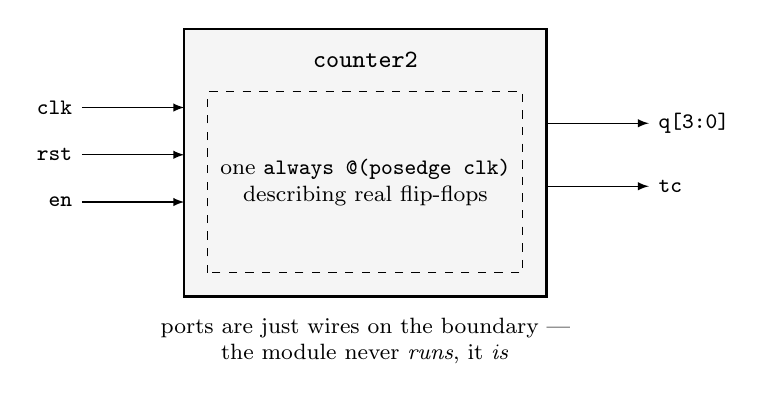
\begin{tikzpicture}[font=\small, >=latex]
  \draw[thick, fill=gray!8] (0,0) rectangle (4.6,3.4);
  \node at (2.3,3.0) {\ttfamily counter2};
  \draw[thin, dashed] (0.3,0.3) rectangle (4.3,2.6);
  \node[align=center, font=\footnotesize] at (2.3,1.45)
    {one \texttt{always @(posedge clk)}\\ describing real flip-flops};
  % input ports
  \foreach \y/\n in {2.4/clk, 1.8/rst, 1.2/en}{
    \draw[->] (-1.3,\y) -- (0,\y);
    \node[left, font=\ttfamily\footnotesize] at (-1.3,\y) {\n}; }
  % output ports
  \foreach \y/\n in {2.2/q[3:0], 1.4/tc}{
    \draw[->] (4.6,\y) -- (5.9,\y);
    \node[right, font=\ttfamily\footnotesize] at (5.9,\y) {\n}; }
  \node[align=center, font=\footnotesize, anchor=north] at (2.3,-0.15)
    {ports are just wires on the boundary ---\\ the module never \emph{runs}, it \emph{is}};
\end{tikzpicture}
